\section{Dialogue Manager}
\subsection{State Automa}
Il professor Piton è stato da noi realizzato come una sorta di automa a stati finiti non deterministo con coda, con i seguenti stati:
\begin{itemize}
    \item[i)]\textbf{Intro}: stato iniziale transitorio necessario solamente per far partire il dialogo con lo studente interrogato;
    \item[ii)]\textbf{Not Useful}: stato ricorrente in cui il professore si accorge che la risposta data dall'utente non è per lui utile. Questo accade quando non vi è riferimento esplicito a pozioni e/o ingredienti oppure quando l'utente propone una domanda. In questo scenario viene generata una frase \textit{filler} con lo scopo di far procedere la conversazione;
    \item[iii)]\textbf{Fill The Frame}: stato ricorrente, complementare al precedente, in cui il professore si accorge che la risposta data dallo studente è utile e va a riempire il frame che sta mantenendo per poi generare la prossima domanda;
    \item[iv)]\textbf{Trabocchetto}: stato ricorrente in cui il professore fa un trabocchetto allo studente suggerendogli un ingrediente di un altra pozione rispetto alla corrente selezionata per l'interrogazione;
    \item[v)]\textbf{Hint}: stato ricorrente in cui il professore fa un suggerimento allo studente chiedendogli se un argomento della pozione sia o meno presente;
    \item[vi)]\textbf{Questions}: stato ricorrente in cui il professore fa domande standard riguardo alla pozione scelta.
\end{itemize}
Per una maggiore comprensione verrà di seguito proposto una schema di transizione degli stati:
\begin{figure}[h]
\centerline{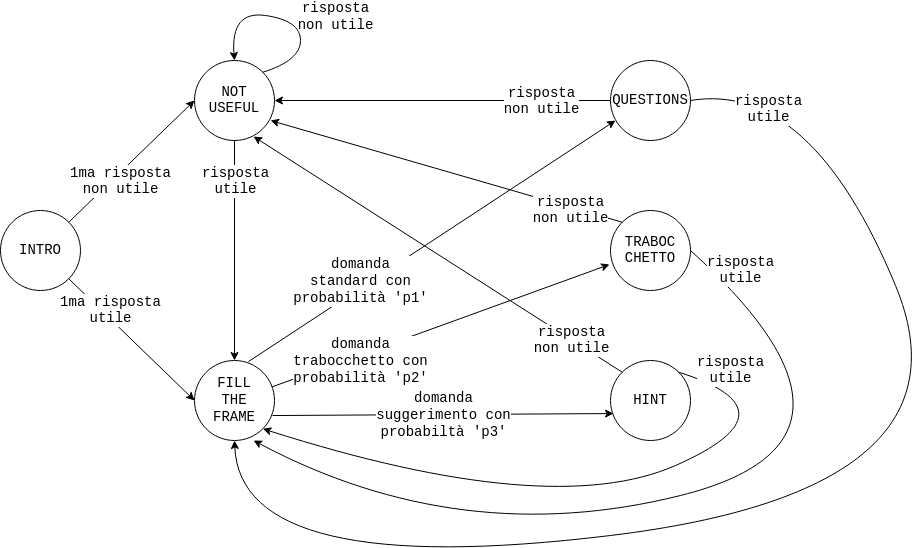
\includegraphics[scale=0.4]{Images/stateTransition.png}}
\caption{Automa di Piton, il non determinismo risiede nella generazione delle domande che sono regolate da distribuzioni di probabilità}
\label{fig:Automa}
\end{figure}

\subsection{Logica Implementativa}
Come già accennato Piton è frame based nel senso che conduce la conversazione, mediante opportune domande, verso informazioni che ritiene necessarie per completare il frame dedicato alla pozione. Nello specifico le domande per essere utili sono rigenerate continuamente fino a quando non si verifica una delle seguenti condizioni:
\begin{itemize}
    \item abbiamo una domanda generica sulla pozione e siamo nello stato \textit{questions};
    \item abbiamo una domanda che contiene un ingrediente di un' altra delle pozioni che ha in memoria e siamo nello stato \textit{trabocchetto};
    \item abbiamo una domanda che contiene un ingrediente della corrente pozione e siamo nello stato \textit{hint}
\end{itemize}
\subsection{Mental State}
Piton è dotato di uno \textbf{stato mentale} scelto tra \textbf{angry}, \textbf{neutral} e \textbf{happy} in maniera probabilistica all'inizio dell'esecuzione. Conoscendo il personaggio cinematografico queste probabilità sono a favore di un cattivo umore, che può però cambiare durante l'interazione se l'utente si dimostra molto ben preparato. Lo stato mentale impatta nell'esecuzione sia nella generazione, facendo affidamento a corpus di generazione completamente diversi e specifici per ogni stato, sia nella valutazione finale. Ad ogni turno di dialogo lo stato mentale può mutare sia in meglio che in peggio tenendo conto degli errori compiuti dall'utente, delle informazioni corrette restituite e della lunghezza della conversazione. 
\subsection{Terminazione}
Il dialogo termina se si presenta una delle seguenti condizioni:
\begin{enumerate}
    \item La conversazione procede per un numero di turni che è 3 volte il numero di ingredienti della pozione;
    \item Il frame viene completato e l'utente ha detto correttamente o no tutti gli ingredienti della pozione.
\end{enumerate}

\subsection{Valutazione}
La valutazione prende in conto tutto quello che è stato detto e genera il voto $v$ con la seguente formula:
\[
v = 31 - \alpha \cdot \textbf{p} \\
\]
31 così parte con la lode, $\alpha$ è il moltiplicatore della penalità $\textbf{p}$ in base al suo stato mentale: $\alpha = 1.5$ se neutrale, $\alpha=2$ se arrabbiato $\alpha = 1$ se felice.
\[
\textbf{p} = \#err + \frac{\#ext + \#plur}{2} + (3\cdot t - 3)
\]
con $\#err$= numero degli errori, $\#ext$= numero degli ingredienti esterni, $\#plur$ = numero dei singolari al posto dei plurali o viceversa e:
\[
t = \frac{\#tentativi fatti}{\# tentativi perfetti}
\]
\newpage
Usiamo la funzione $y = 3x -3$ per trattare il precedente rapporto perchè ragionevole e facile da calcolare:
\begin{figure}[h]
\centerline{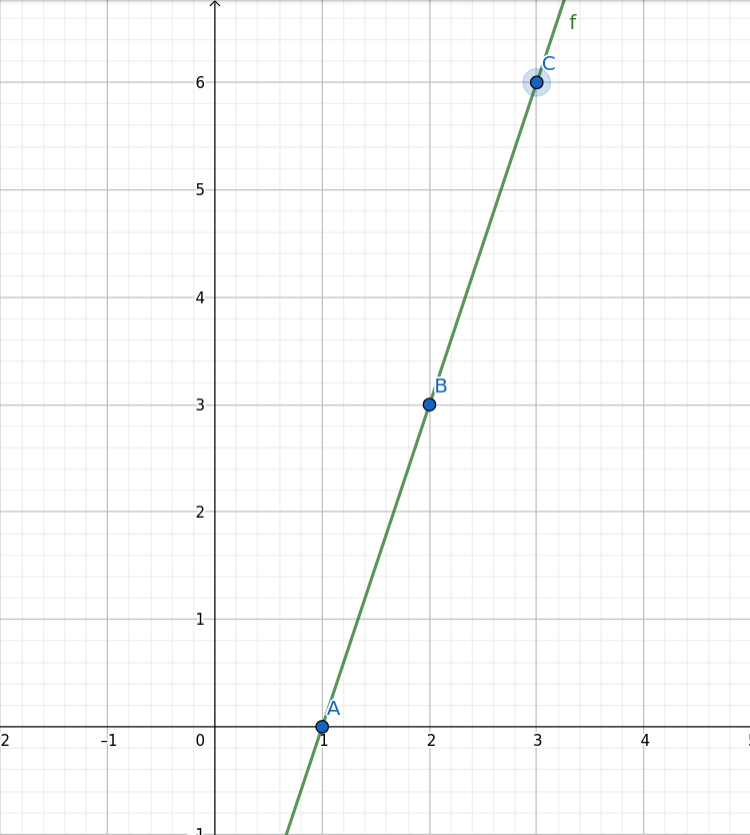
\includegraphics[scale=0.25]{Images/3x-3.png}}
\caption{Grafico della funzione $y = 3x -3$}
\label{fig:FunzioneVoto}
\end{figure}

Se i tentativi sono minimi ($t=1$) non c'è penalità, se invece lo studente risponde nel doppio dei tentativi ($t=2$) togliamo 3 punti fino a 6 punti per il triplo ($t=3$) delle risposte necessarie.
\newline
Mettendo tutto assieme risulta:
\[
v = 31 - \alpha \cdot (\#err + \frac{\#ext + \#plur}{2} + (3\cdot t - 3))
\]
